\documentclass[12pt]{article}
\usepackage[utf8]{inputenc}
\usepackage{amsmath}
\usepackage{color,lineno,setspace,multirow}
\usepackage{graphicx}
\usepackage[top=2.4cm,left=2.4cm,top=2.4cm,bottom=2.4cm,includefoot]{geometry}
\usepackage{natbib}
\usepackage{caption}
\usepackage{pdflscape}

% TODO
% complete the figures for the graphical interpretation
% legends
% perform simulations
% finish writing the first draft


\bibliographystyle{bes}

\begin{document}

\linenumbers
\modulolinenumbers[1]

\textbf{Title:} Should ecological interactions influence diversification rates in ecological networks?\\

\textbf{Authors:} Dominique Gravel$^{1,2,*}$, Timothée Poisot$^{2,3}$, Marie-Josée Fortin$^{4}$, Kevin Cazelles$^{2,5}$, Paulo Guimaraes$^{6}$, David Hembry$^{7}$ \\

\textbf{1}: Canada Research Chair in Integrative Ecology. Département de
biologie, Université de Sherbrooke, 2500 Boulevard l'Université,
Sherbrooke (Québec). J1K 2R1\\
\textbf{2}: Québec Centre for Biodiversity Science\\
\textbf{3}: Université de Montréal, Département des Sciences Biologiques, 90 Avenue Vincent d’Indy, Montréal, QC H2V3S9, Canada.\\
\textbf{4}: \\
\textbf{5}: \\
\textbf{6}: \\
\textbf{7}: \\
* corresponding author at dominique.gravel\@usherbr

\textbf{Keywords:} networks, macro-evolution, island biogeography, predator-prey, mutualism, competition; 

\textbf{Words in the abstract: } \\ 
\textbf{Words in the main text: } \\
\textbf{Words in the legends: } \\

Authorship: 

\newpage
\doublespacing

%=============================================================================%
\section*{Abstract}

\newpage

%=============================================================================%
\section*{Introduction}

Competitive interactions are widely considered to be dominant in governing the
ecological and evolutionary dynamics of biodiversity on earth. Extensive
empirical evidence demonstrates that competitive interactions govern the use
of resources by species in communities (e.g., Lotka-Volterra, Tilman 1982;
Diamond and Case 1986), the mechanism of natural selection (e.g., Darwin 1859;
Simpson 1953), character displacement and adaptive radiation (Brown and Wilson
1956; Schluter 2000a,b; Losos 2009). In evolutionary biology, competition has
been widely invoked to explain species richness across time and space (see
review in Rabosky 2013). Competition among species and clades for finite
resources (e.g., “ecological limits”) is thought to impose carrying capacities
on species diversity, and thus diversity-dependent diversification (Rabosky
2013). Compelling evidence exists that supports the view that diversity-
dependent processes operate to regulate patterns of biodiversity at local,
regional, and continental scales. This includes lack of a correlation
between clade age and species richness (Ricklefs and Renner 1994;
Rabosky 2012; Rabosky et al. 2012); evidence from the fossil record of
stable diversity through time at local (Knoll 1986; Wing and
DiMichele 1995; DiMichele et al. 2004; Cleal et al. 2012) and global scales
(Spekoski 1978, 1984; Alroy 2010a,b; Smith et al. 2012; but see Benton and
Emerson 2007; Friedman and Sallan 2012; Lloyd and Friedman 2012); and,
most controversially, some evidence from the branching patterns of molecular
phylogenies (see discussion and references in Rabosky 2013).

Substantial evidence indicates that diversity-dependence of diversification
rates are likely real in many cases, but substantial evidence questioning its
primacy exists as well. Not all studies examining diversity through time find
support for this view in molecular phylogenies, with some studies arguing that
such data are consistent with or mask continuously increasing (Morlon et al.
2010; Manceau et al. 2015) or declining diversity trajectories (Quental and
Marshall 2010; Morlon et al. 2011). Furthermore, molecular phylogenetic
studies apparently consistent with density-dependence might alternately
reflect a pattern of some clades undergoing increases in diversity and others
decreases at any given point in time (Pyron and Burbrink 2012; Rabosky et al.
2012). The same is true for the fossil record, where there is substantial
disagreement over whether patterns of standing diversity through time are
consistent with ecological limits; certainly, over deep time, global patterns
of diversity (e.g., Sepkoski 1978, 1984) are variously described as consistent
with nonequilibrial fluctuations in diversity or a “stepped logistic” increase
(see review in Harmon and Harrison 2015). It is possible that some of these
examples simply represent exceptional cases — such as the subset of clades that
have recently diversified into new adaptive zones (Simpson 1953; Rabosky and
Hurlbert 2015). Furthermore, the boundary between the sets of conditions under
which competition promotes diversity (e.g., through character displacement, or
the ecological theory of adaptive radiation; Lack 1947; Simpson 1953; Brown
and Wilson 1956; Schluter 200a,b) and constrains diversity (e.g., clade
competition, ecological limits over macroevolutionary timescales; Simpson
1953; Jablonski 2008; Rabosky and Glor 2010; Pires et al. 2015) are not well-
understood (Hembry et al. 2014; but see Bailey et al. 2013).

More importantly, in our view, the investigation of whether macroevolutionary
dynamics are consistent with density-dependence and/or ecological limits on
diversity have overlooked the fact that not all ecological interactions among
species are competitive. Antagonistic interactions — particularly predator-
pre y— have attracted substantial attention from paleobiologists, some of whom
have emphasized the difficulty of distinguishing the effects of competition
from those of predation (Dietl and Kelly 2002; Stanley 2008). In some
evolutionary radiations, the two are likely intermixed (REF). Integrating
mutualism into this macro-evolutionary theory has been more challenging,
although a number of authors have argued that mutualism provides novel
resources to interacting clades, thus providing ecological opportunity and
spurring diversification (Lengyel et al. 2009; Gómez and Verdú 2012; Litsios
et al. 2012; Joy 2013). It is certainly conceivable that competition trumps
all other interactions, both because of global resource limitation and because
mutualistic and antagonistic interactions often contain a component of
interspecific competition within trophic levels for prey or mutualistic
partners (Ehrlich and Raven 1964; Schluter 2000; Armbruster and Muchhala
2007). However, it is also possible that the effects of competition on
diversity dynamics are substantially modulated by other ecological
interactions, such as mutualism and predation.

SOMETHING MISSING HERE TO MOTIVATE A NETWORK APPROACH TO MACRO-EVOLUTION

Here, we introduce a simple model of competitive interactions in a natural
community can, and through extensions to mutualistic and antagonistic
predator-prey interactions, can generate easily interpretable predictions as
to the effects of different types of interactions on mecroevolutionary
diversity dynamics. In some cases, these predicted dynamics differ between
competition and other types of ecological interactions, suggesting that mixed
empirical evidence for diversity-dependence and ecological limits on diversity
over evolutionary time may be due in part to the effects of antagonism and
mutualism on diversity.

%=============================================================================%
\section*{Graphical model of diversification dynamics}

We start with a graphical model of speciation-extinction dynamics inspired by
the theory of island biogeography and its recent extensions to include trophic
interactions and other types of ecological networks (Gravel2011; Cazelles2015;
Massol2017). The model allows to derive some basic predictions about the
imapct of different types of interactions on diversification rates. Its
simplicity however prevents the investigation of the macroevolution of network
structure, and we thus relax some assumptions and perform numerical
simulations below.

%------------------------
\subsection*{Description} 

The rate of change in species richness $R$ is a dynamic balance between
speciation events and extinction events, represent as follows:

\begin{equation}
	\frac{dR}{dt}\frac{1}{R} = S(R) - E(R)
\end{equation}

where $S(R)$ is the function describing the speciation rate as a function of
species richness, and $E(R)$ the extinction rate. The equilibrium species
richness is found when $S(R) = E(R)$. A minimal birth-death model of macro-
evolution is species-richness independent, such that $S$ and $E$ are constant
rates $s$ and $e$. We observe exponential diversification provided that $s>e$
. More recent models use phenenological representation of the diversification
dynamics, such as:

\begin{equation}
	\frac{dR}{dt}\frac{1}{R} = (s-e)(1 - \frac{R}{K})
\end{equation}

where $s$ and $e$ are baseline speciation and extinction rates, and $K$ is the
maximal species richness the system can support. This approach could be
sufficient to describe the dynamics of the system and test hypotheses, but it
does not allow to understand the underlying ecological mechanisms fixing
carrying capacity. It could not discriminate for instance the effect of
various types of interactions, or if the constraints are imposed by
coexistence or decreasing population size. Here we propose a general model
with simple functions describing how ecological interactions could modify the
speciation and extinction rates under different scenarios of ecological
interactions.

Our derivation is inspired by the trophic theory of island biogeography
(Gravel2011), which add redator-prey interactions to the MacArthur \& Wilson
model of colonization and extinction dynamics without the addition of extra
parameters. Ecological interactions are introduced with a simple assumption:
predators require a prey to colonize islands and persist. If the last prey
goes extinct, then there is secondary extinction of the predator (Dunne2002).
The derivation is based on the computation of the expected number of preys a
predator has on the island. As a first approximation, if the island holds $R$
species and the connectance of the ecological network is $C$, then the
expected number of interacting species is simply $I = CR$. Our subsequent
derivation is based on this expected number of interacting species with the
resident and newly speciated species. The exact formulation requires knowledge
of interactions and species co-occurrence (see Cazelles2015), but the
approximation holds for general predictions as we will see below with
numerical simulations.

The key to develop the model further and investigate different types of
interactions is to define the functions $S(R)$ and $E(R)$ appropriately.   We
consider a successful speciation event to be the combination of a mutation
leading to speciation and the acquisition of traits that are ecological
suitables (i.-e. they provide preys, mutualists or minimize competition). In
what follows we use exponential equations for these functions, but other
functional forms could be considered as well, depending on the assumptions
considered. Thus, we define:

\begin{equation}
	S(R) = u_{max}(u_0 + u_1 e^{-\alpha I})
\end{equation}

and 

\begin{equation}
	E(R) = e_{max}(e_0 + e_1 e^{-\alpha I})
\end{equation}


where $u_{max}$ and $e_{max}$ are the asymptotic speciation and extinction
rates respectively, and $u_1-u_0$ and $e_1-e_0$ are the speciation and
extinction rates in absence of interactions. There are multiple ways to
parameterize those functions, for different types of interactions. These are
summarized at Table 1 and the functions are illustrated at Fig. 1-3. In short,
interactions are modifiers of the $u_{max}$ and $e_{max}$ and the shape of the
function depends on the type of interactions. Maximal speciation rate could
happen either at null diversity (e.g. in absence of interactions) or at
infinite interactions (e.g. with mutualism).

%------------------------
\subsection*{Competition}

Competition could impact both speciation rate, because it could limit the
establishment of mutants, and extinction rate because it decreases population
size and therefore promotes stochastic extinction. We consider that a
successful speciation event is limited by the availability of ecological
niches (i.-e. there is a limiting similarity setting a cap to species richness
- MacArthur1967). At this stage we do not represent niches explicitly, but
simply assume that niche space is filled asymptotically with increasing
species richness. Therefore, the speciation rate is maximal at $I = 0$, which
means that $u_1-u_0 = u_{max}$ and it decreases progressively as the number of
competitors increase. We consider that it tends asymptotically to 0 with
species richness approxing very large numbers (i.e. $u_0 = 0$). Alternatively,
intense competition could also result in exclusion of already established
species, either because mutants are more performant or because of reduced
population size. We consequently consider that the extinction probability is
minimal at $I = 0$ and increases asymtotatically with $I$ to a maximal
extinction probability $e_{\infty} = e_{max}$.

%------------------------
\subsection*{Mutualism}

Mutualism could impact the speciation rate because newly speciated species
require partners to establish their mutualism. The probability of finding at
least one partner already present in the community, and the total benefit from
all partners, should increase with the expected number of interactions. We
consequently consider that the speciation rate is minimal at $I = 0$, with the
extreme case of obligate mutualism where $u_1-u_0 = 0$, and it saturates at
the maximal speciation rate $u_0 = u_{max}$. At the opposite of competition,
mutualism increases population size and fitness, such that the extinction rate
is expected to decrease asymptotatically with the number of interactions. We
consequently set the extinction probability in absence of interactions at the
max $e_1-e_0 = e_{max}$, with the extreme case of obligate mutualism where
$e_{max}=1$, and the asymptote to $e_0 = e_{min}$. This last probability is
larger than 0 because extinctions independent of interactions could
nonetheless occur. Note this model applies to mutualistic interactions as well
as ammensalism (+,0).

%------------------------
\subsection*{Predator-prey interactions}

Predator-prey interactions combine the negative effect of interactions on
extinction described for competition with the positive effect of mutualists on
colonization described for mutualism. We consider that successful speciation
of a predator require to find at least one prey to establish. The speciation
function should thus be increasing and saturating with species richness, as it
is for mutualism. The extinction function is however more complicated, as it
combines two different constraints. First, there increasing benefit of having
multiple preys since the likelihood of all preys going extinct should decrease
with species richness. Second, predatory interactions could have a negative
impact on the prey, reducing there density and potentially leading to
extinctions. Depending on the relative importance of these two functions, the
final extinction probability could be a monotonic decreasing and asymptotic
function of the expected number of interactions, or alternativel it could have
a fast decrease followed by an increase of the extinction rate (such as
illustrated at Fig. X). In this last situation, there is an initial reduction
of extinction probability because of beneficial preys, followed by an increase
because of harmful effects of predators.

%------------------------
\subsection*{Results} 

A graphical representation of the speciation and extinction curves allow one
to understand the impact of different types of interactions on diversification
dynamics. An equilibrium $\hat{R}$ exists at the location where the $S(R)$ and
the $E(R)$ curves cross each other (Fig. 1A). The shape of the curves tells us
about the stability of the equilibrium and the diversification dynamics, which
could be stable or not. Species richness will increase when $S(R) > E(R)$ and
conversely, it will decrease when $S(R) > E(R)$. Diversification dynamics will
be stabilizing if $S(R) < E(R)$ when species richness is larger than the
equilibrium $\hat{R}$ (species richness decreases) and $S(R) > E(R)$ when
species richness is smaller than the equilibrum. The opposite leads to
exponential diversification dynamics.

The simple analysis of this graphical model reveals that competitive
interactions will limit species diversification if the speciation and
extinction curves cross each other (Fig. 1). Given the above described
assumptions for the shape of the speciation and extinction functions, we find
there is only one equilibrum and it will always be stable. The consequent per
species diversification rate will be a monotonic negative relationship with
species richness, which shape will depend on the assumptions underlying the
$S(R)$ and $E(R)$ functions.

Mutualistic interactions on the other hand are susceptible to unbounded
diversification (Fig. 2). In contrast with competitive interactions, the
speciation and the extinction curves could cross but the equilibrium species
richness will be unstable and per species diversification rate will accelerate
with increasing species richness. In this situation, an increase of species
richness above the equilibrium will result in a speciation rate higher than
the extinction rate, and so diversity will increase without boundaries. The
per species net diversification rate will consequently be a positive monotonic
function of species richness. Alternatively, insufficient initial species
richness could lead to a collapse of the system.

Predator-prey interactions combine the findings of both competitive and
mutualistic interactions. The speciation function follows the same shape to
the mutualistic function. The extinction function on the other hand could take
various forms, with various outcomes. The most interesting case is a hump-
shape relationship, susceptible to cross the speciation curves twice,
generating potentially two equilibrium points (Fig. 3). The first equilibrium
$\hat{R}_1$ is unstable. In this case, if species richness is below the
equilibrium, speciation will be insufficient to balance extinctions and the
system will collapse. If the initial species richness is larger than this
point, then species richness will increase and reach the second equilibrium,
which is stable. Species richness will decrease if starting from higher
species richness than the second equilibrium. The shape of the extinction
curve will determine wether only one or two equilibrium will be found. The
shape depends on the relative rates of change of the extinction functions for
the effects of prey (more preys decrease extinctions) and predators (more
predators increase extinctions). If the decay parameters $\alpha$ are similar,
then the function will be a negative exponential and there will be a single
stable equilibrium. Two equilibrium will be found when the positive effect of
preys saturates much faster than the negative effect of predators.

%=============================================================================%
\section*{Simulation of network macro-evolution}

%------------------------
\subsection*{Description}

The graphical model yields very general conclusions about the impact of
different types of interactions on diversification dynamics, but it does not
allow the investigation of network macro-evolution, thereby neglecting any
impact of network topology on its development. Therefore, in addition to the
simple analytical model, we run stochastic simulation with a more explicit
representation of ecological interactions. The analytical model considers that
all species interact similarly (they have on average the same number of
interactions) and that the role of the species in the network (Stouffer2012)
does not influence diversification dynamics. Previous work on the TTIB shown
this approximation to be valid to understand the broad principles of spatial
food web dynamics, but that a more realistic representation of trophic
position and species role does influence occupancy (Gravel2011; Massol2017).
In addition to these limitations, the inheritance of traits and the
consequently progressive building of the network is susceptible to impact
diversification rate (Romanuk2017). For instance, in a predator-prey system, a
top carnivore with trophic level 4 requires at least the presence of
herbivores and inferior carnivores to establish. The probability of a
successful speciation event toward a top predator will therefore increase with
species richness, much later than for herbivores.

Speciation and extinction probabilities are computed exactly as described
above for the analytical model, except that $I$ is extracted from the
knowledge of the interaction network. We therefore need to model the macro-
evolution of this network and the role of each species in it. We couple the
speciation-extinction model described above with a network model describing
interactions as a function of a set of evolving traits for each species. We
adopt the formalism of the niche model of food web interactions
(Williams2000), extended to represent as well competitive and mutualistic
interactions.

Each species is characterized by a set of traits defining their niche.
Competition, mutualistic and predator-prey interactions differ by the rules
that are set to relate the optimum and the range to the niche position. For
simplicity, we consider univariate competition networks and bipartite
mutualistic networks. In both cases, species have a niche position $n_i$ and a
niche range $r_i$. A species $i$ interact with other species $j$ whose niche
position falls within the range $[n_i - r_i, n_i + r_i]$. In addition for
predator-prey interactions, because the interactions are directed, each
species has a niche position $n_i$ and an optimum $o_i$. A predator with niche
position $n_i$ feeds on preys whose niche position $n_j$ falls within the
range $[o_i - r_i, o_i + r_i]$.

Different rules determine sampling of traits for initial ancestral species and
their mutants $m$. At the start of a simulation, for all three types of
interactions, niche position is drawn at random from a uniform distribution
bounded between 0 and 1. For simplicity and to avoid the evolution of super
generalists (there are no explicit trade-offs giving costs to generality), the
range is drawn from a beta distribution with an average $E[r] = 0.2$ and a
shape parameter $\beta_{r}$. The optimum is drawn from a beta distribution
with mean $E[o] = \gamma_0 + \gamma_1n$ and shape parameter $\beta_{o}$. This
constraint imposes a relationship between niche position, range and optimum
inspired by the relationship between predator and prey body size (Gravel2013).

Mutants inherit traits from their ancestors. The niche position is drawn from
the beta distribution with an average $E[n]_i$ and a shape parameter
$\beta_{n}$. The shape parameter determines the spreading around the average
trait value and thus controls the innovation at each mutation event. This
trait is the only one to evolve. The range is fixed for all three scenarios.
The optimum is deterministically determined from the new niche position. The
difference between the expected niche optimum given the niche position is
transposed to the new niche optimum. In other words, the niche optimum of the
mutant is given by the equation $o_M = E[o_M] + (E[o_A] - o_A)$, where
$E[o_i]$ is the expected optimum given the niche position, as described above.

%------------------------
\subsection*{Results}


%=============================================================================%
\section*{Discussion}

\begin{itemize}
\item summary of the main conclusions

\item the reality can't be any of these extreme cases

\item is there any partial support for any of these interpretations ? Can we use the predictions to revisit some classical studies ?  

\item what are the additional predictions to test ? 
%    - clade age frequency distribution ?
%    - age vs trophic level ? 
%    - age vs specialization ? 

\end{itemize}    
%========================================================%
\section*{Conclusion}

%========================================================%
\section*{Acknowledgements} 

This is a contribution to the working group Space and time variation of ecological networks, support by the NIMBIOS. 

\newpage

%========================================================

%\bibliography{library}
%\newpage

%========================================================%

%\begin{landscape}
\begin{table}[]
%\centering
\caption{Summary of model parameters and values used for figures 1-3}. The (-) sign for the extinction function indicates the negative Extinction-Richness relationship and the (+) sign indicates the positive relationship. Connectance was set at 0.1 for all figures.

\begin{tabular}{lllll}
\hline
Variable & Name & Competition & Mutalism & Predation \\
\hline
$u_{max}$ 		& Maximal speciation rate 				& 0.5	& 		& 		\\ 
$u_{0}$			& Asympotic speciation rate 			& 0		& 		& 		\\
$u_{1}$			& Speciation rate at null richness 		& 0.5	& 		& 		\\
$e_{max}$		& Maximal extinction rate 				& 1		& 		& 		\\
$e_{0-}$		& Asymptotic extinction rate (-) 		& 0.2	& 		& 		\\
$e_{1-}$		& Extinction rate at null richness (-) 	& 0.1	& 		& 		\\
$e_{0+}$		& Maximal speciation rate (+) 			& NA	& 		& 		\\
$e_{1+}$		& Maximal speciation rate (+)			& NA	& 		& 		\\
$\alpha_{u}$	& Decay of $S(R)$ function 				& 0.1	& 		& 		\\
$\alpha_{e-}$	& Decay of $E(R)$ function for - 		& 0.1	& 		& 		\\
$\alpha_{e+}$	& Decay of $E(R)$ function for +		& NA	& 		& 		\\
\hline
\end{tabular}
\end{table}
%\end{landscape}

\newpage

%========================================================%
\section*{Figure legends}

%------------------------
\subsection*{Figure 1}

\textbf{Graphical interpretation of the diversification dynamics with competitive interactions}. The vertical dotted line indicate the equilibrium species richness. Arrows points in the direction of the dynamics when the system is out of equilibrium species richness. All parameters are provided at Table 1. 

%------------------------
\subsection*{Figure 2}

\textbf{Graphical interpretation of the diversification dynamics with mutualistic interactions}. All parameters are provided at Table 1. 

%------------------------
\subsection*{Figure 3}

\textbf{Graphical interpretation of the diversification dynamics with predator-prey interactions}. All parameters are provided at Table 1. 

%------------------------
\subsection*{Figure 4}

\newpage

%========================================================%

%------------------------
\subsection*{Figure 1}

\begin{figure}[ht!]
\centering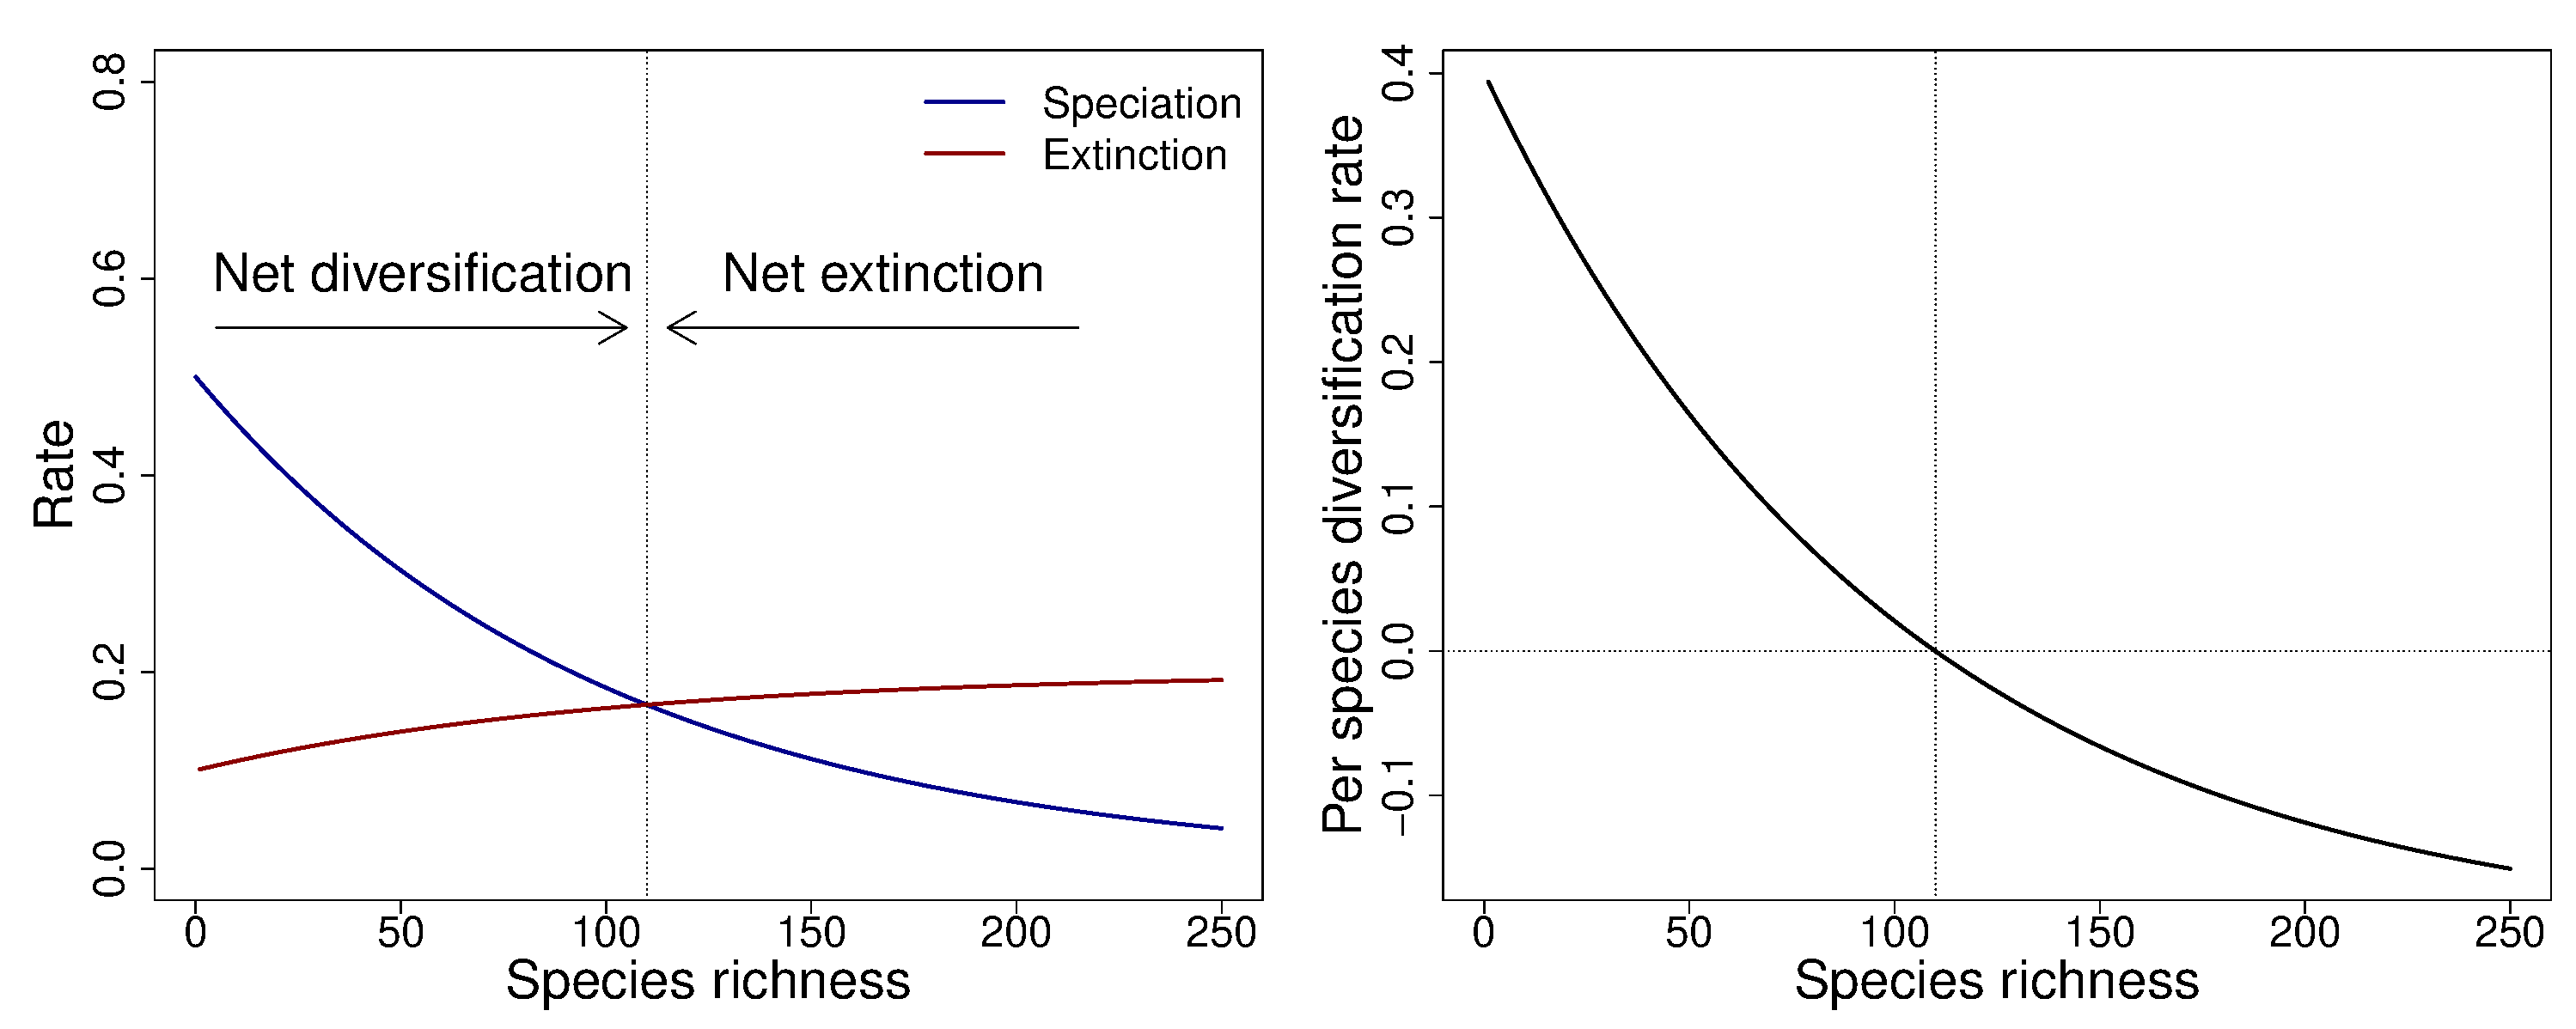
\includegraphics[width=1\textwidth]{figures/competition}
\end{figure}

\newpage

%------------------------
\subsection*{Figure 2}

\begin{figure}[ht!]
\centering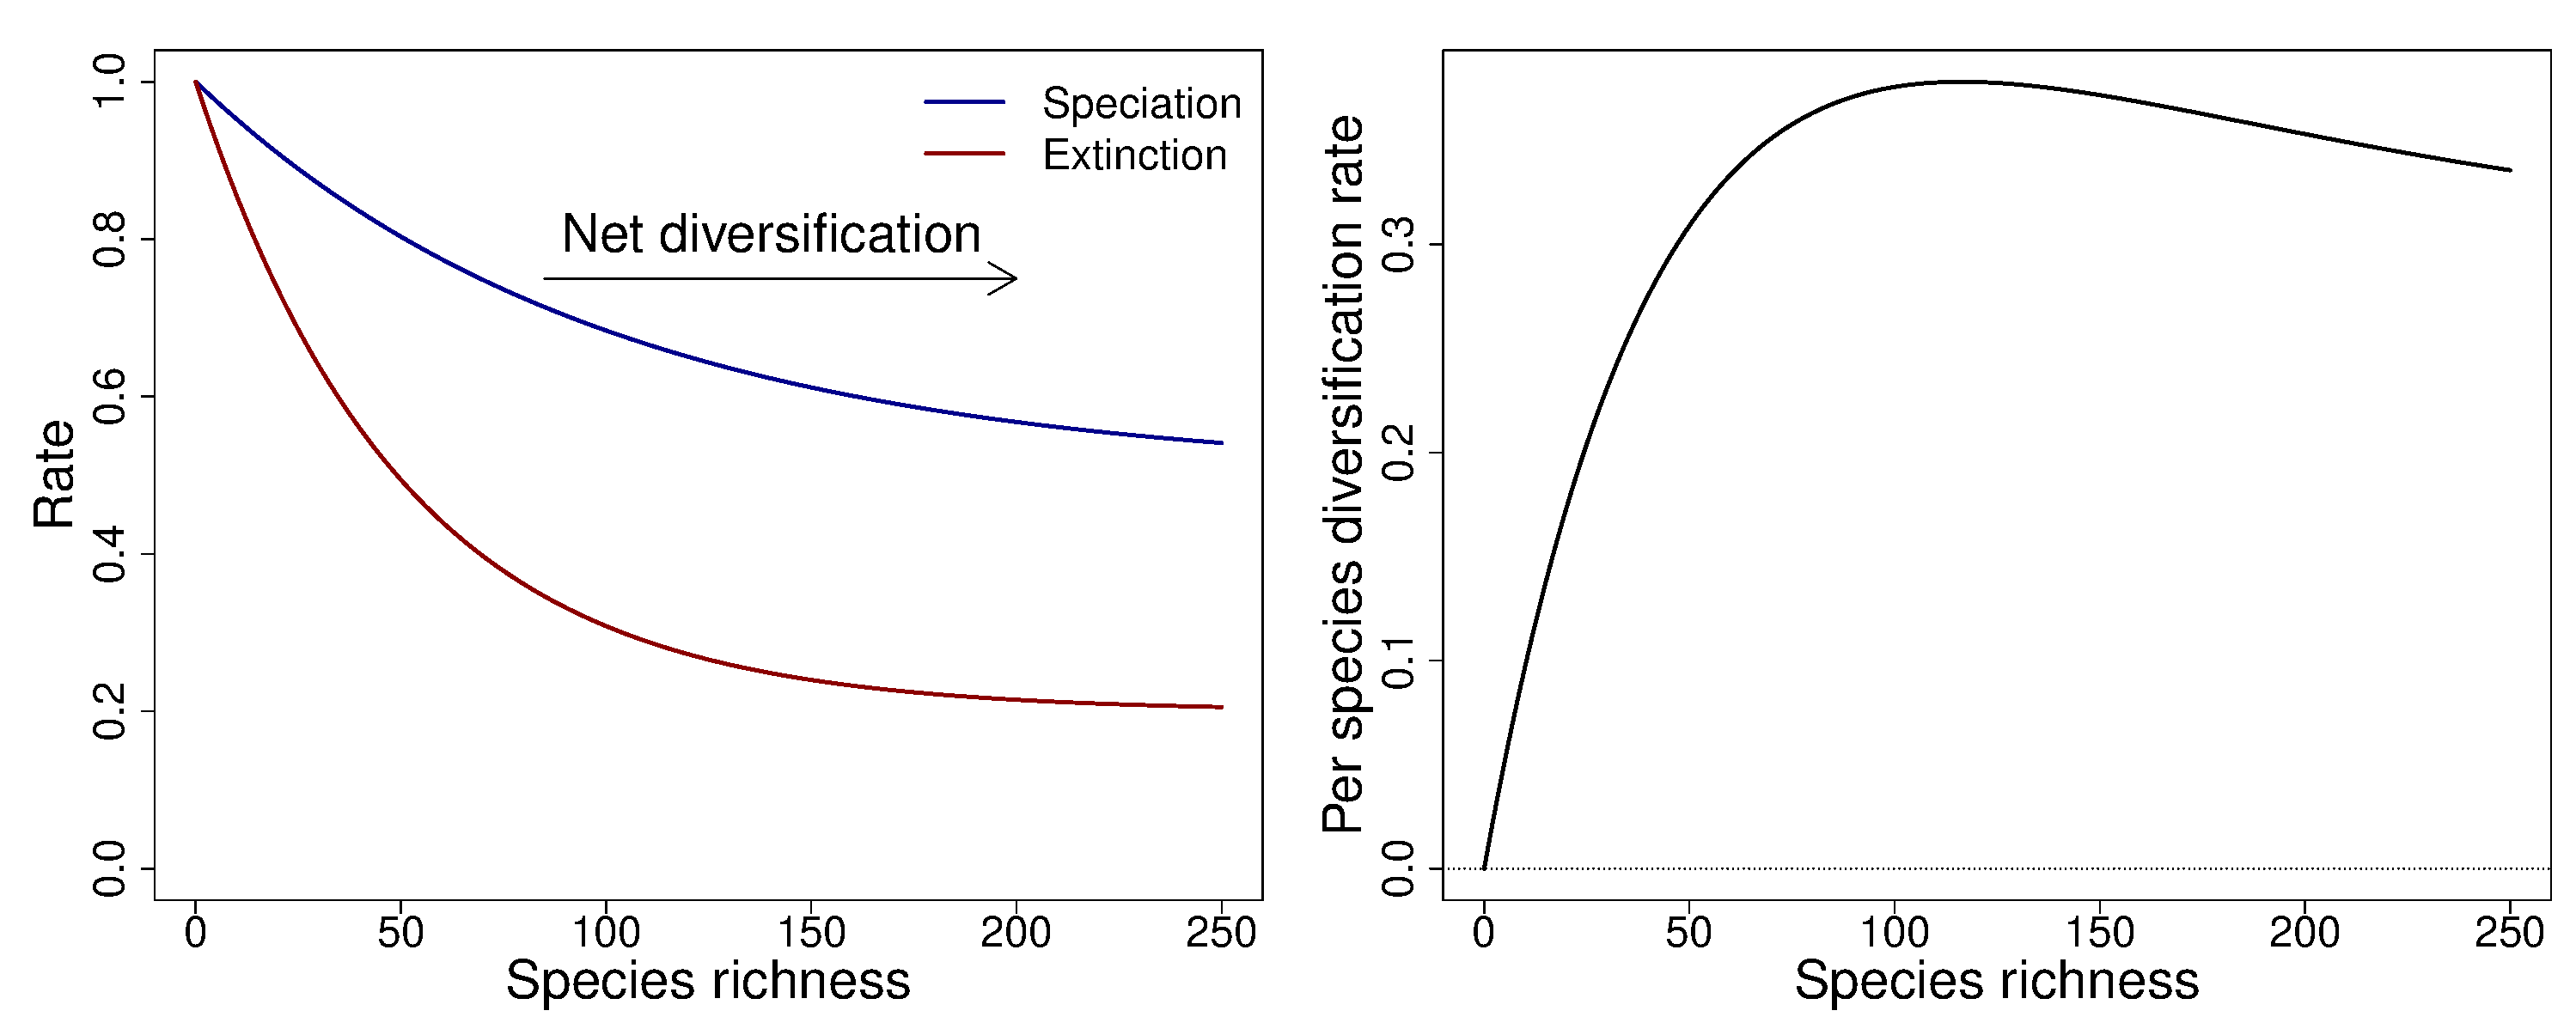
\includegraphics[width=1\textwidth]{figures/mutualism}
\end{figure}

\newpage

%------------------------
\subsection*{Figure 3}

\begin{figure}[ht!]
\centering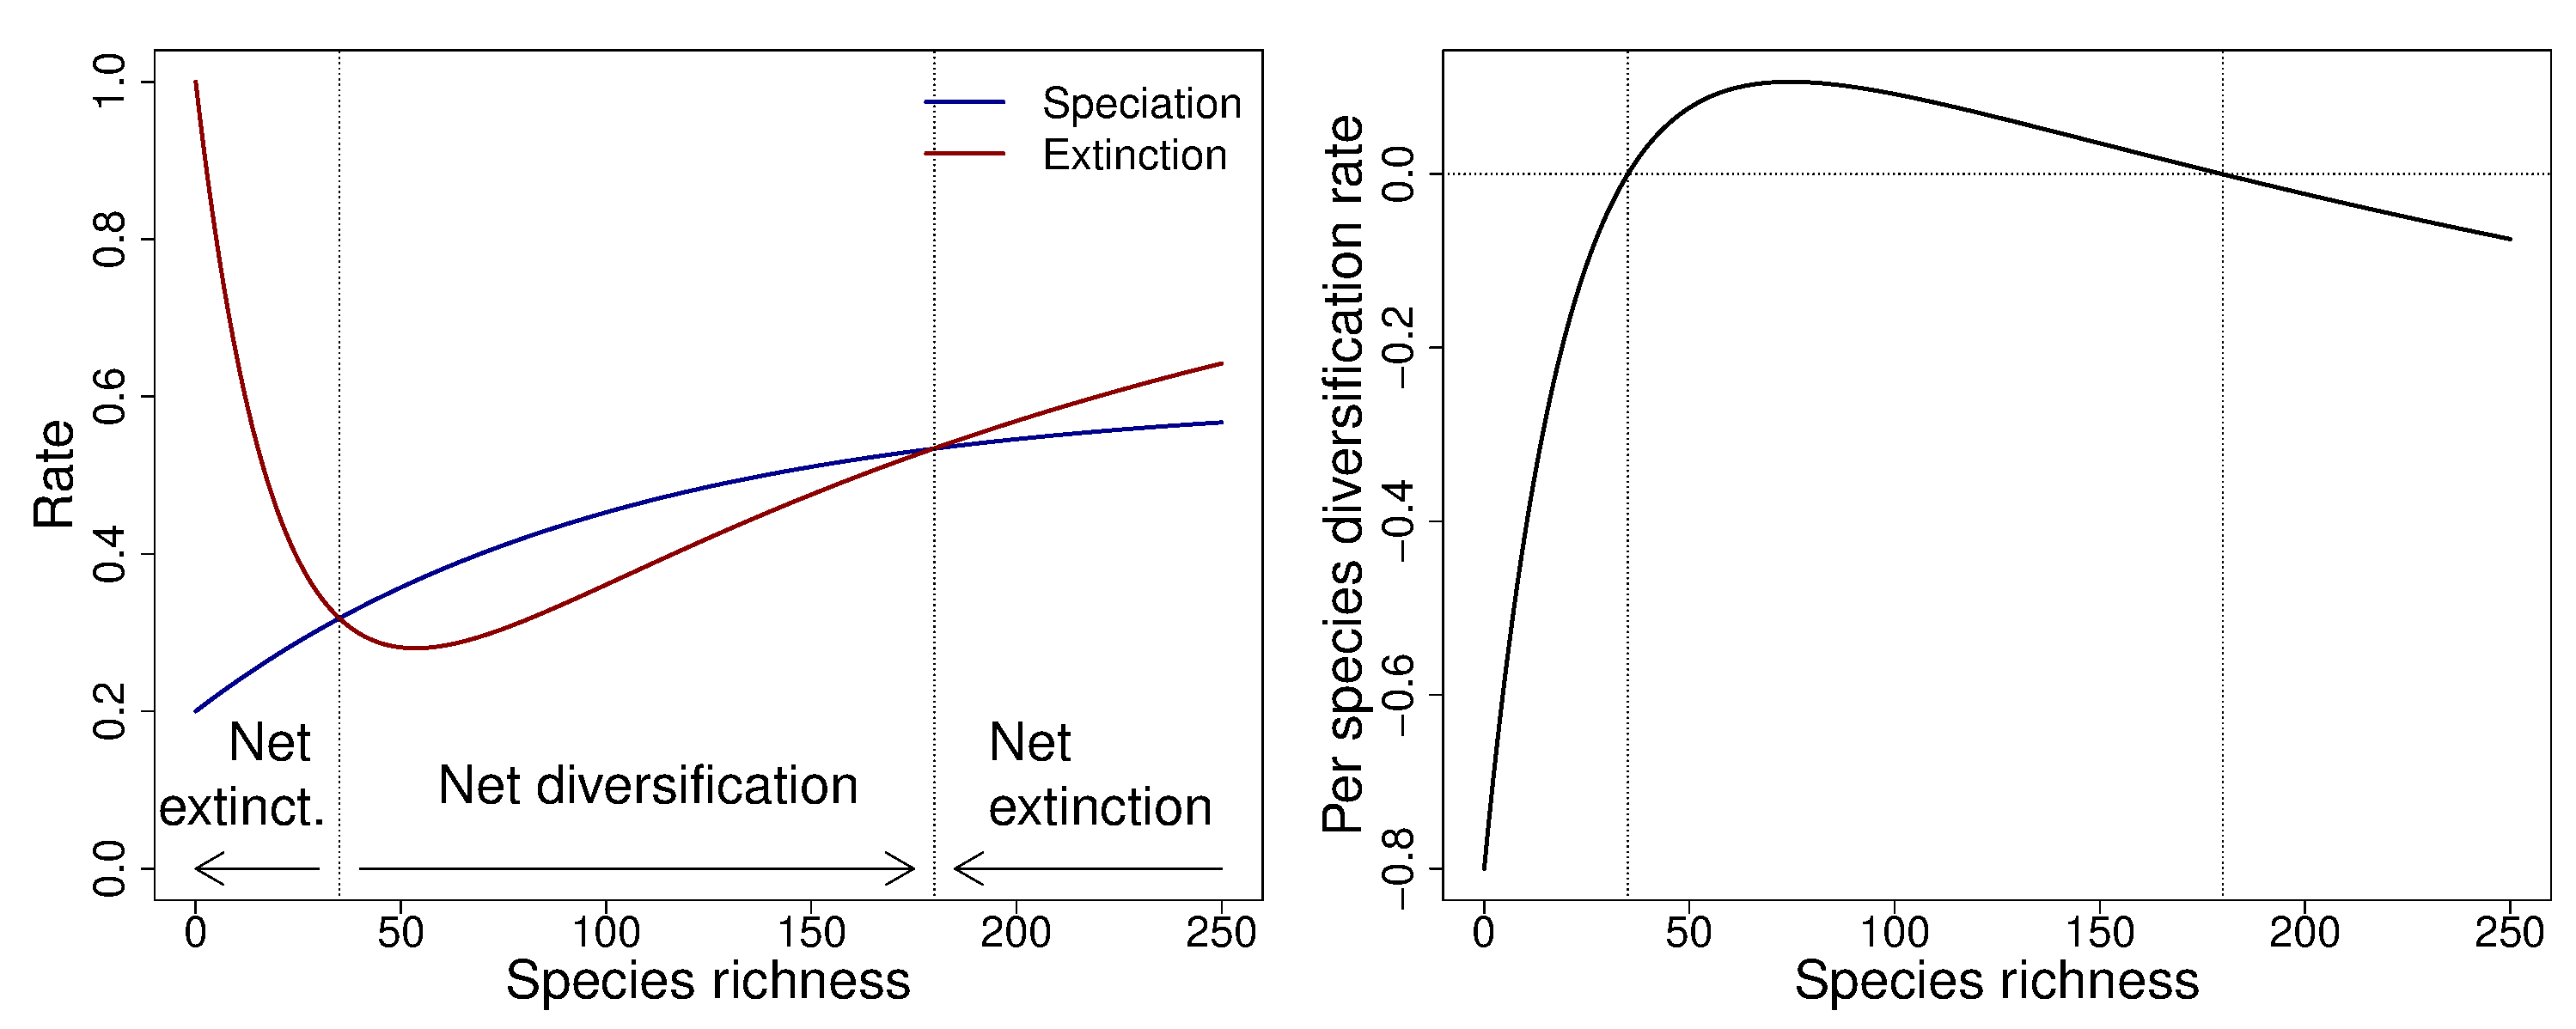
\includegraphics[width=1\textwidth]{figures/predation}
\end{figure}

\newpage

%------------------------
\subsection*{Figure 4}

\begin{figure}[ht!]
\centering\includegraphics[width=0.8\textwidth]{figures/simulations}
\end{figure}

\newpage


%========================================================%
\end{document}
